\begin{figure}[t!]
  	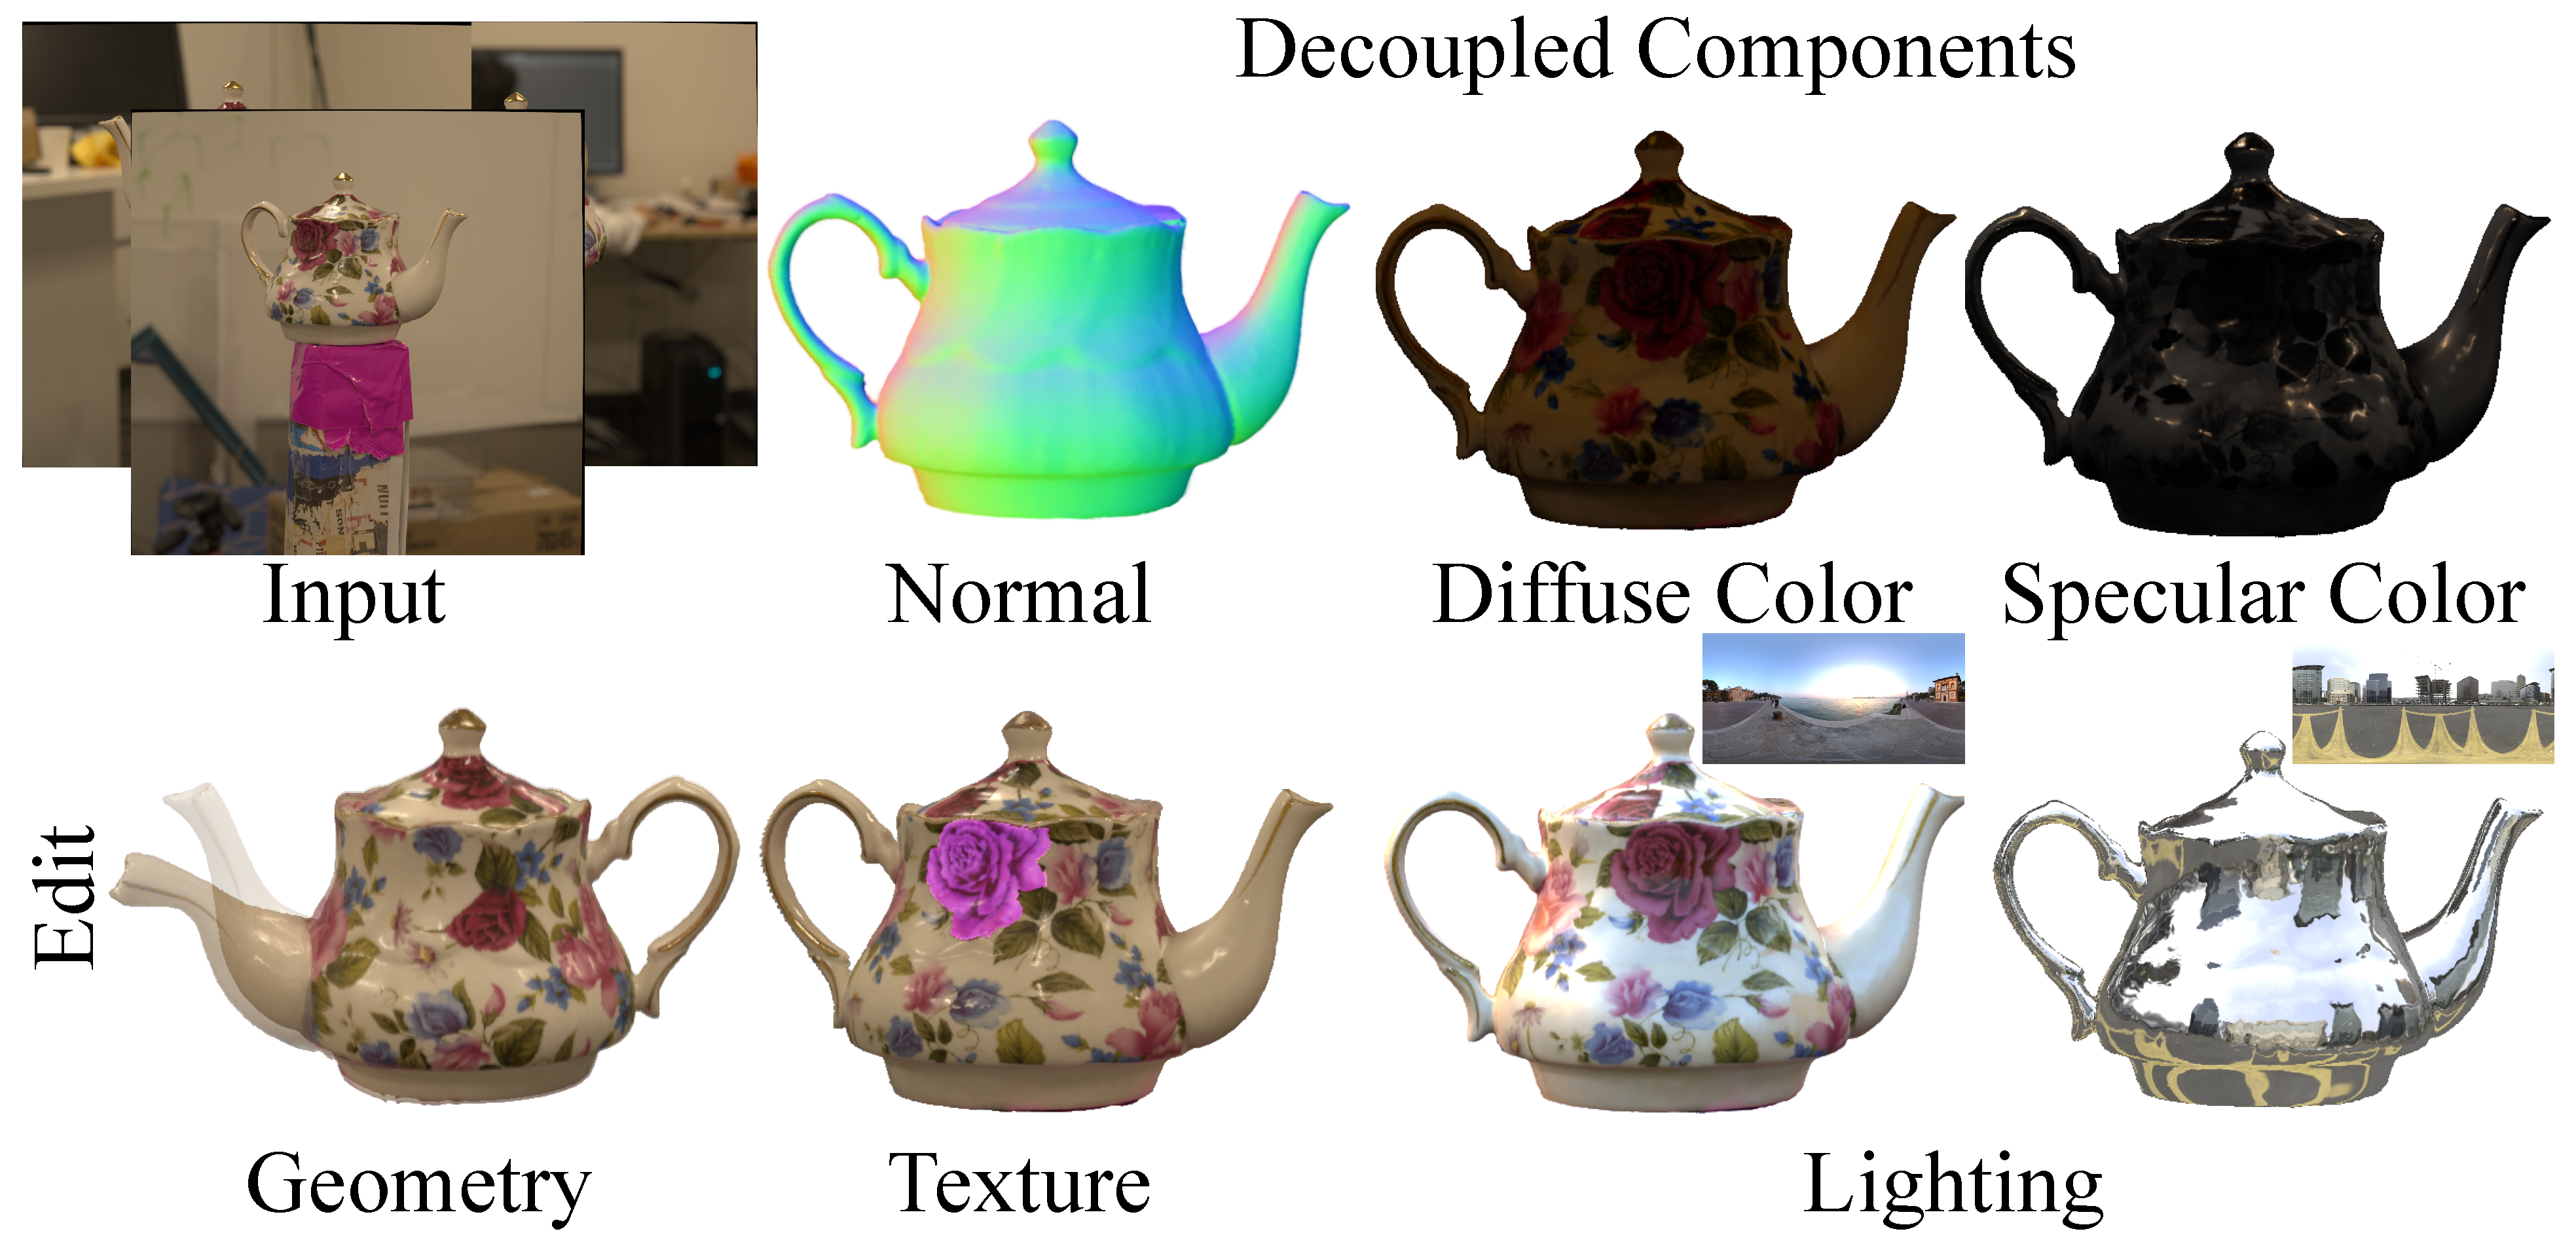
\includegraphics[width=0.99\linewidth]{./img/teaser_teapot_scene001}
    \vspace{-1mm}
    \caption{
        Given multi-view images, \name optimizes a \yl{Gaussian} splatting representation with decoupled geometry, texture, and lighting. 
        With this decoupled representation, \name not only allows geometry and texture editing, but \yl{can also} render the input scene (the 3rd column, bottom row) or the edited scene (the last column, bottom row) under a novel illumination. 
    }
    \vspace{-5mm}
    \label{fig:teaser}
\end{figure}

